%% bip results
We evaluated \deadlocktool{} using several case studies including the dining philosopher example and multiple instances
of a configurable generalized {\em Resource Allocation System} that comprises 
a configurable multi token-based scheduler.
The different configurations of our resource allocation system subsume problems like the Milner's scheduler, 
data arbiters and the dining philosopher with a butler problem. 
We benchmarked the performance of \deadlocktool{} against DFinder on two benchmarks: 
{\em Dining Philosopher} with an increasing number of philosophers and 
a deadlock free resource allocation system with an increasing number of clients and resources. 
%We provide both benchmarks at \href{http://}{}.

All experiments were conducted on a machine with Intel (R) $8$-Cores (TM) $i7$-$6700$, CPU @ $3.40$GHZ, $32$GB RAM, 
running a CentOS Linux distribution. 

\subsubsection{Dining philosophers case study} 
We consider the traditional dining philosopher problem as depicted in 
Figure~\ref{fig:diningSpectrum}.
The Figure shows $n$ philosophers competing on $n$ forks modeled in BIP. 

Each philosopher component has $2$ states, and each fork component has $3$ states. 
Thus, The total number of states is $2^n \times 3^n$. 
We evaluated \deadlocktool{} by increasing $n$ and applying both $\LAO$ and $\LLin$ methods and compared against the best configuration 
we could compute with DFinder2. 
DFinder2 allows for several techniques to be applied. The most efficient one is 
the Incremental Positive Mapping (IPM) technique \cite{DFinder2}. 
IPM requires a manual partitioning of the system to exploit its efficiency. 
We applied IPM on all structural partitions and we report on the best result which is consistent 
%(takes less time possibly for hardware related reasons) 
with the results reported in \cite{DFinder2}. 

Table~\ref{bench:dining} shows the results. Both $\LAO$ and $\LLin$ outperform the best performance of DFinder2 by several orders of magnitude 
for $n\leq 3,000$. Both $\LAO$ successfully completed the deadlock freedom check for $3,000 \leq n \leq 10,000$ 
in less than one minute, where DFinder2 timed out (~1 Hour). $\LLin$ required $62$ seconds for $n=10,000$. 


Even though $\LLin$ is asymptotically more efficient than $\LAO$,
$\LAO$ outperforms $\LLin$ in all cases. This due to the following. 

\begin{itemize}
\item The largest subsystem that $\LAO$ had to consider was with depth $\l=1$. This corresponds to $18 = 2^1\times 3^2$ states regardless of $n$, the number of philosophers. 
\item The largest subsystem that $\LLin$ had to consider was with depth $\l=2$. This corresponds to $648 = 2^3 \times 3^4$ states regardless of $n$. 
\item For a given depth $\l$, \LLin is more efficient to compute than $\LAO$. 
 Since $\LAO$ performs a stronger check, it often terminates for smaller depths which makes it effectively more efficient than $\LLin$. 
\end{itemize}


\begin{table}
\tbl{Benchmarks: Dining Philosopher}{
\begin{tabular}{| l | l | l | l |}
\hline
Size & \LAO & \LLin & D-Finder \\ \hline \hline
$1,000$ &         $0.46 s$  &   $0.7 s$       & $15 s$ \\ \hline
$2,000$ &          $1.4 s$  &   $1.9 s$       & $60s$ \\ \hline
$3,000$ &          $2.9 s$  &    $4$       & $2m:41s$ \\ \hline
$4,000$ &          $4.8 s$  &    $7$        & $5m:37s$ \\ \hline
$5,000$ &          $8.3 s$  &    $12$        & $12m:38s$ \\ \hline
$6,000$ &          $13.0 s$ &    $17$         & $17m:48s$ \\ \hline
$7,000$ &          $17.2 s$ &   $25$        & $30m:18s$ \\ \hline
$8,000$ &          $25.6 s$ &   $34$        & $-$ \\ \hline
$9,000$ &          $34.1 s$ &   $55$        & $-$ \\ \hline
$10,000$ &          $47 s$  &   $62 s$          & $-$ \\ \hline 
\end{tabular}}
\label{bench:dining}
\end{table}



\subsubsection{Resource allocation system case studies}

We evaluated \deadlocktool{} with a multi token-based resource allocation system. 
The system consists of $n$ clients, $m$ resources, $k$ tokens. 
The number of tokens specifies the maximum number of resources that
can be in use at a given time. 
The system allows to specify conflicting resources. 
Only one resource out of a set of conflicting resources can be in use at a given time.
For each set of conflicting resources, we create a resource manager.
Resource managers are connected in a ring where they pass tokens to neighboring resource managers or to resources. 

Given configuration specifying $n$, $m$, $k$, a map of requests between clients and resources, and a set of sets of conflicting resources, 
we automatically generate a corresponding BIP model.

Figures~\ref{fig:client},
~\ref{fig:resource}, and
~\ref{fig:conflict-token}
show BIP atomic components for client, resource and manager components. 

The client in Figure~\ref{fig:client} requests resources $R_0$ and $R_2$ in sequence. It has $5$ ports. 
Ports $SR_0$ and $SR_2$ send requests for 
resources $R_0$ and $R_2$, respectively.
Ports $RG_0$ and $RG_2$ receive grants for 
resources $R_0$ and $R_2$, respectively.
Port $rel$ releases all resources. 
The behavior of the client depends on its request sequence. 

\begin{figure}[H]
\begin{center}
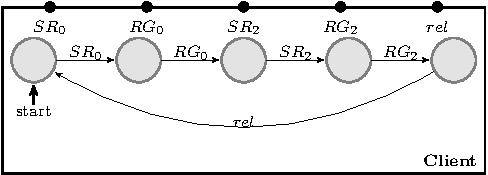
\includegraphics[scale=1.2]{compiledfigures/client-crop.pdf}
\caption{Client}
\label{fig:client}
\end{center}
\end{figure}

Figure~\ref{fig:resource} shows a resource component. 
A resource component waits for a request from a connected client on port $RR$. 
Once a request is received, the resource component transitions to a state where it is ready to 
receive a token from the corresponding resource manager using port $RTT$.
The resource transitions to a state where it grants the client request using port $STC$ and waits until it is released on port $done$. 
There, it returns the token back to the resource manager and transitions to the start state. 

\begin{figure}[H]
\begin{center}
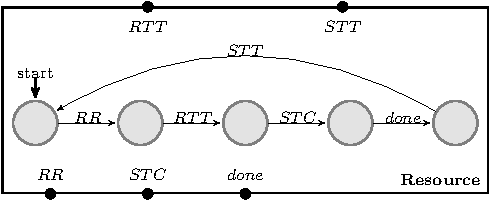
\includegraphics[scale=1.2]{compiledfigures/resource-crop.pdf}
\caption{Resource}
\label{fig:resource}
\end{center}
\end{figure}

Figure~\ref{fig:conflict-token} shows a resource manager.
A resource manager $M$ has four states. 
\begin{itemize}
  \item State $T$ denotes that $M$ has a token. $M$ may send the token to either 
    (1) a resource on port $STR$ and transition to state $TwR$ (token with resource), or 
    (2) the next resource manager on port $STT$ and transition to state $N$ (no token).
  \item State $N$ denotes that $N$ has no token. 
    It may receive a token from a neighboring resource manager in the ring on port $RTT$ 
    and transition to state $T$. 
  \item State $TwR$ denotes that $M$ has already passed a token to one of its resources. 
    $M$ may either receive (1) the assigned token back from the resource using port $RTR$ and transition to state $T$, 
    or (2) another token from a neighboring manager using port $RTT$ and transition to state $TTwR$ (token and token with resource).
  \item State $TTwR$ denotes that $M$ has a token and has already passed a token to one of its resources. 
    In this state $M$ can not send the token it has to a resource it manages to respect the conflict constraint. 
    $M$ may send the token to the next manager on port $STT$ and transition back to state $TwR$. 
\end{itemize}

\begin{figure}[H]
\begin{center}
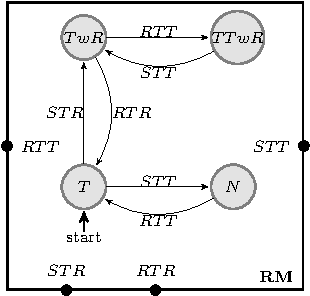
\includegraphics[scale=1.2]{compiledfigures/token-crop.pdf}
\caption{Token Resource Manager}
\label{fig:conflict-token}
\end{center}
\end{figure}

The connections between a resource manager $M$ and its resources on ports $STR$ and $RTR$ specify that the 
resources are conflicting. 
A system should have at least $x$ resource managers where $x$ is the maximum between the number of sets of conflicting resources 
and $k$.
Note that $k$ resource managers start at state $T$ to denote the $k$ tokens; the rest start at state $N$. 

Figure \ref{fig:resourceallocation} shows a configuration system with $5$ clients and $5$ resources where:
\begin{itemize}
  \item Client $C_0$ requires resource $R_0$ then $R_2$,
  \item Client $C_1$ requires resource $R_2$ then $R_0$,
  \item Client $C_2$ requires resource $R_1$,
  \item Client $C_3$ requires resource $R_3$, and
  \item Client $C_4$ requires resource $R_4$.
\end{itemize}

The system has three resource managers to specify the conflicting resources. 
$RM_{01}$ manages conflicting resources $\{R_0,R_1\}$. 
$RM_{23}$ managers conflicting resources $\{R_2,R_3\}$.
$RM_{4}$ manages resource $R_4$. 

\begin{figure}[H]
\begin{center}
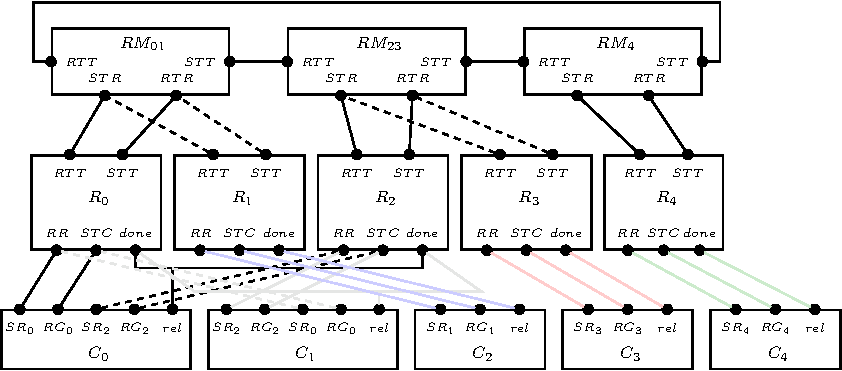
\includegraphics[scale=0.9]{compiledfigures/resourceallocation-crop.pdf}
\caption{Conflict-Resource Allocation System}
\label{fig:resourceallocation}
\end{center}
\end{figure}

We evaluated \deadlocktool{} with various configurations.
We highlight several lessons learned for specific systems as follows. 

\paragraph{Lesson 1:} 
$\LAO$ verifies freedom from global and local deadlock where DFinder2 can only verify freedom from global deadlock.
Consider a system with $5$ clients, $3$ tokens, and $5$ resources.
Clients request resources $\langle 0, 2\rangle, \langle 2, 0\rangle, \langle 1 \rangle, \langle 3\rangle,$ and $\langle 4\rangle$, respectively.
Resource sets $\{ 0, 1\}, \{2,3\}$ are conflicting. 
This system clearly is a global deadlock free. 
It has a local deadlock where client $C_0$ has resource $0$ and client $C_1$ has resource $2$. 
DFinder qualitatively can not detect such a local deadlock while $\LAO$ successfully does. 

\paragraph{Lesson 2:} 
$\LAO$ is more complete than both $\LLin$ and DFinder2. For example, it can verify global and local deadlock freedom in cases where $\LLin$ fails. 
Consider a system with $5$ clients, $2$ tokens, and $5$ resources.
Clients request resources $\langle0, 2\rangle, \langle 0, 2\rangle, \langle 1 \rangle, \langle 3\rangle,$ and $\langle 4\rangle$, respectively.
Resource sets $\{ 0, 1\}, \{2,3,4\}$ are conflicting. 
This system is global and local deadlock free. 
Both DFinder2 and $\LLin$ report that the system might contain a deadlock. 
$\LAO$ successfully reports that the system is both global and local deadlock free. 

\paragraph{Lesson 3:}
Our work can be extended to detect conspiracies \cite{AFG93}.
For example, consider a system with
$5$ clients, $2$ tokens, and $5$ resources.
Clients request resources $\langle 0, 1\rangle, \langle 1, 0\rangle, \langle 2 \rangle, \langle 3\rangle,$ and $\langle 4\rangle$, respectively.
Resource sets $\{ 0, 1\}, \{2,3,4\}$ are conflicting. 
Client $C_0$ may block forever in case it acquires resource $0$ because resource $0$ is conflicting with resource $1$. 
However, it is not possible to find a deadlocked subsystem containing $C_0$ and resources $0$ and $1$ since that will also have
to include the resource manager $M_{01}$ managing conflicting resources $0$ and $1$. 
The latter can always exchange the second token with the neighboring resource managers. 

An extension of our work that consider subsystem boundaries at ports and abstracts port enablement 
conditions with free Boolean variables can help
detect such scenarios. 

\begin{table}
\tbl{Benchmarks: Time required for $\LAO$ on the resource allocation system}{
\begin{tabular}{| l | 
  c |  c | c | c | 
  c |  c | c | c | 
  c |  c | c |  }
\hline

Size & $10$ & $12$ & $14$ & $16$ & $18$ & $20$ & $22$ & $24$ & $26$ & $28$ & $30$ \\ \hline
Time (sec) & $148 $ & $169 $ & $189 $ & $230 $ & $254 $ & $277 $ & $298 $ & $318 $ & $351 $ & $374 $ & $430 $ \\ \hline 

\end{tabular}}
\label{bench:resourceallocation}
\end{table}

\paragraph{Benchmarking:}

We evaluated the performance of $\LAO$ on a deadlock free system with the following configuration. 
\begin{itemize}
\item $n$ clients each with $3$ states, $n$ resources each with $5$ states, and $n$ tokens,
\item Client $C_i, 0\leq i < n$ requests resource $i$, and 
\item No resources are in conflict, hence we have $n$ resource managers each with $4$ states. 
\end{itemize}

The system has a total of $4^n \times 3^n \times 5^n$ states. 
DFinder2 timed out within seven hours for $n=10$. 
%Try different combinations of partitions
$\LLin$ had to increase the subsystem up to the whole system and also timed out within seven hours for $n=10$. 
$\LAO$ was able to verify deadlock freedom. It has to check subsystems with $12$ components out of $3\times n$ components regardless of $n$. 
This resulted from inspecting subsystems corresponding to a depth $\l=2$ with $\leq 23,040,000=4^{6} \times 3^2\times 5^4$ states regardless of $n$.
The numbers in Table~\ref{bench:resourceallocation} show a linear increase in time required to check deadlock freedom 
using $\LAO$ with respect to $n$. This indicates that the number of subsystems to check is proportional to $n$. 

Our resource allocation system subsumes the token based Milner scheduler~\cite{milner} which 
is essentially a token ring with precisely one token present~\cite{AGR16}. 
The technique presented in ~\cite{AGR16} fails to prove deadlock freedom for Milner Scheduler 
because it requires a large subset of the system, 
while $\LAO$ succeeds. 
